%To compile as handout, use
%pdflatex "\def\ishandout{1} \input{filename.tex}"
%Defaults to non-handout mode (with slide reveals)
\ifdefined\ishandout
  \documentclass[handout]{beamer}
\else
  \documentclass{beamer}
\fi
 
\usepackage{econ103slides} 

\date{Lecture 23}


\begin{document} 




%%%%%%%%%%%%%%%%%%%%%%%%%%%%%%%%%%%%%%%%

\begin{frame}[plain]
	\titlepage 
	

\end{frame} 

%%%%%%%%%%%%%%%%%%%%%%%%%%%%%%%%%%%%%%%%%
\begin{frame}
\begin{block}
	{Experiment}
	\begin{itemize}
		\item Weigh a known 10 gram mass 16 times on the same scale.
		\item Scale makes normally distributed measurement errors:
		$X_1, \hdots, X_{16} \sim \mbox{iid } N( \mu, \sigma^2 = 4)$
	\end{itemize}
\end{block}
\begin{alertblock}
			{Measurement Errors?}
		 Weigh same object repeatedly $\Rightarrow$ slightly different result each time. Average deviation from mean $\approx 2$ grams.
		\end{alertblock}
\begin{block}{Two Kinds of Scales}
	\begin{description}
			\item[Unbiased] Correct on average: $\mu = 10$ grams
			\item[Biased] \emph{Too high} on average: $\mu = 11$ grams
		\end{description}	
		
\end{block}

\end{frame}

%%%%%%%%%%%%%%%%%%%%%%%%%%%%%%%%%%%%%%%%

\begin{frame}
	\frametitle{An Idea for Deciding if a Scale is Biased}

\begin{enumerate}
	\item Test $H_0 \colon \mu = 10$ against $H_1\colon \mu > 10$ with $\alpha =0.025$.
	\item Decide based on the outcome of test:
		\begin{itemize}
	\item Reject $H_0 \Rightarrow$ decide scale is biased, throw it away.
	\item Fail to reject $H_0 \Rightarrow$ decide scale is unbiased, keep it.
			\end{itemize}	
\end{enumerate}

\end{frame}
%%%%%%%%%%%%%%%%%%%%%%%%%%%%%%%%%%%%%%%%
\begin{frame}[t]
	\frametitle{Testing Whether a Scale is Biased \hfill 
\includegraphics[scale = 0.05]{./images/clicker}}
	\fbox{$X_1, \hdots, X_{16} \sim \mbox{iid } N( \mu, \sigma^2)$ where we \emph{know} $\sigma^2 = 4$}

	\vspace{2em}

	Suppose I want to test $H_0\colon \mu = 10$. What is my test statistic? 

	\vspace{1em}

	\begin{enumerate}[(a)]
		\item $4\bar{X}/S$  
		\item $4(\bar{X} - 10)/S$
		\item $(\bar{X} - \mu)/(S/\sqrt{n})$
		\item $2 \bar{X}$
		\item $2(\bar{X} - 10)$ 
	\end{enumerate}

	\pause
	\alert{$$T_n = \frac{\bar{X} - \mu_0}{\sigma/\sqrt{n}} = \frac{\bar{X} - 10}{2/\sqrt{16}} = 2(\bar{X} - 10)$$}
\end{frame}
%%%%%%%%%%%%%%%%%%%%%%%%%%%%%%%%%%%%%%%%
\begin{frame}[t]

	\frametitle{Testing Whether a Scale is Biased \hfill 
\includegraphics[scale = 0.05]{./images/clicker}}
	\fbox{$X_1, \hdots, X_{16} \sim \mbox{iid } N( \mu, \sigma^2)$ where we \emph{know} $\sigma^2 = 4$}

	\vspace{2em}

	What is the sampling distribution of $2(\bar{X}-10)$ under $H_0\colon \mu = 10$? 

	\vspace{1em}

	\begin{enumerate}[(a)]
		\item $N(\mu, 4)$  
		\item $N(0, 4)$  
		\item $t(15)$  
		\item $\chi^2(15)$  
		\item $N(0,1)$  
	\end{enumerate}

	\pause
	\alert{$H_0\colon \mu = 10 \implies \displaystyle T_n = \frac{\bar{X} - \mu_0}{\sigma/\sqrt{n}} =  2(\bar{X} - 10)\sim N(0,1)$}
\end{frame}
%%%%%%%%%%%%%%%%%%%%%%%%%%%%%%%%%%%%%%%%

\begin{frame}[t]
	\frametitle{Testing Whether a Scale is Biased \hfill 
\includegraphics[scale = 0.05]{./images/clicker}}
	\fbox{$X_1, \hdots, X_{16} \sim \mbox{iid } N( \mu, \sigma^2)$ where we \emph{know} $\sigma^2 = 4$}

	\vspace{1em}

	Suppose I want to test $H_0\colon \mu = 10$ against the \emph{one-sided} alternative $\mu > 10$ with $\alpha = 0.025$. What is my decision rule? 

	\vspace{1em}

	\begin{enumerate}[(a)]
		\item Reject $H_0$ if $2(\bar{X} - 10) > 1$ 
		\item Reject $H_0$ if $2(\bar{X} - 10) < 1$ 
		\item Reject $H_0$ if $2(\bar{X} - 10) > 2$ 
		\item Reject $H_0$ if $2(\bar{X} - 10) < 2$ 
		\item Reject $H_0$ if $|2(\bar{X} - 10)| > 2$ 
	\end{enumerate}

	\pause
	\alert{Reject $H_0$ if $T_n = 2(\bar{X} - 10) >$ \texttt{qnorm(1 - 0.025)} $\approx 2$}
\end{frame}
%%%%%%%%%%%%%%%%%%%%%%%%%%%%%%%%%%%%%%%%
\begin{frame}
	\frametitle{Testing an \emph{Unbiased} Scale\hfill 
\includegraphics[scale = 0.05]{./images/clicker}}
	 Unbeknownst to me the scale I am testing is in fact \emph{unbiased}.
	 What is the probability that I will decide, based on the outcome of my test, to throw it away?

	 \vspace{2em}
	\pause

	\alert{This is simply a Type I Error! Hence the probability is $\alpha = 0.025$}
\end{frame}
%%%%%%%%%%%%%%%%%%%%%%%%%%%%%%%%%%%%%%%%
\begin{frame}
	\frametitle{Testing a \emph{Biased} Scale\hfill 
\includegraphics[scale = 0.05]{./images/clicker}}
	 Unbeknowst to me the scale I am testing is in fact \emph{biased}.
	 What is the probability that I will decide, based on the outcome of my test, to throw it away?

\pause

\vspace{1em}

\alert{This is the \emph{opposite} of a Type II error...}
\end{frame}
%%%%%%%%%%%%%%%%%%%%%%%%%%%%%%%%%%%%%%%%
\begin{frame}
	\frametitle{What is the probability of throwing away a \em{biased} scale?}

	\begin{block}
		{Decision Rule}
		Decide scale is biased if $2(\bar{X} - 10) > 2$ or \emph{equivalently} if \alert{$\bar{X} > 11$} 
	\end{block}
	\begin{block}
		{Biased Scale}
		$\mu = 11 \quad \implies \quad X_1, \hdots, X_{16} \sim \mbox{iid } N(11, \sigma^2 = 4)$
	\end{block}
	\begin{alertblock}
		{Which implies...}
	\end{alertblock}
\end{frame}
%%%%%%%%%%%%%%%%%%%%%%%%%%%%%%%%%%%%%%%%
\begin{frame}
	\frametitle{Testing a \emph{Biased} Scale\hfill 
\includegraphics[scale = 0.05]{./images/clicker}}

	Suppose $X_1, \hdots, X_{16} \sim N(11, \sigma^2 = 4)$. What is the sampling distribution of $\bar{X}$?
	
	\vspace{1em}

	\begin{enumerate}[(a)]
		\item $N(11, 1)$
		\item $N(0, 1)$ 
		\item $t(15)$
		\item $N(11, 1/4)$ 
		\item $N(10, 1/4)$
	\end{enumerate}
\pause

\vspace{1em}

\alert{$$\bar{X}_n \sim N(\mu, \sigma^2/n) = N(11, 1/4)$$}
\end{frame}
%%%%%%%%%%%%%%%%%%%%%%%%%%%%%%%%%%%%%%%%
\begin{frame}
	\frametitle{What is the probability of throwing away a \em{biased} scale?}

	\begin{block}
		{Decision Rule}
		Decide scale is biased if $2(\bar{X} - 10) > 2$ or \emph{equivalently} if \alert{$\bar{X} > 11$} 
	\end{block}
	\begin{block}
		{Biased Scale}
		$\mu = 11 \quad \implies \quad X_1, \hdots, X_{16} \sim \mbox{iid } N(11, \sigma^2 = 4)$
	\end{block}
	\begin{alertblock}
		{Which implies}
		$\bar{X} \sim N(11, 1/4)\quad \implies \quad$  \alert{$P(\bar{X}>11) = 1/2$} 
	\end{alertblock}

\vspace{1em}

	\alert{\fbox{The \emph{power} of this test is 50\%}}
\end{frame}
%%%%%%%%%%%%%%%%%%%%%%%%%%%%%%%%%%%%%%%%
\begin{frame}[c]\frametitle{Recall:}

\begin{block}
	{Type I Error} Rejecting $H_0$ when it is true:  $P(\mbox{Type I Error}) = \alpha$
\end{block}

\begin{block}
	{Type II Error} Failing to reject $H_0$ when it is false: \alert{$P(\mbox{Type II Error}) =\beta$}
\end{block}

\begin{alertblock}
	{Statistical Power} The probability of rejecting $H_0$ when it is false: \alert{$\mbox{Power} = 1 -\beta $}\\ i.e.\ the probability of \emph{convicting} a guilty person.
\end{alertblock}

\vspace{1em}

\begin{center}
\alert{\boxed{
\begin{minipage}
	{0.95\textwidth}
	Hypothesis tests are designed to control Type I error rate ($\alpha$). But we also care about Type II errors. What can we learn about these?
\end{minipage}}}
\end{center}
\end{frame}
%%%%%%%%%%%%%%%%%%%%%%%%%%%%%%%%%%%%%%%%
\begin{frame}
	\frametitle{Recall: Normal Population Known Variance}
	\begin{block}
		{Sampling Model}
		$X_1, \hdots, X_n \sim N(\mu, \sigma^2)$ where $\sigma^2$ is known
	\end{block}
	\begin{block}
		{Sampling Distribution}
		$$\frac{\bar{X}_n - \mu}{\sigma/\sqrt{n}} \sim N(0,1)$$
	\end{block}
	\begin{block}
		{Under $H_0\colon \mu = 0$}
		$$T_n = \frac{\bar{X}_n}{\sigma/\sqrt{n}} \sim N(0,1)$$
	\end{block}
\end{frame}

%%%%%%%%%%%%%%%%%%%%%%%%%%%%%%%%%%%%%%%%
\begin{frame}
	\frametitle{What happens if $\mu \neq 0$?}
	\begin{alertblock}
		{Key Point \#1}
		\begin{itemize}
			\item Test Statistic $T_n=\sqrt{n}(\bar{X}_n/\sigma)$
			\item Unless $\mu = 0$, test statistic is \emph{not} standard normal!
			\item When $\mu \neq 0$, distribution of $T_n$ \emph{depends on} $\mu$!	
		\end{itemize}
	\end{alertblock}
	\begin{alertblock}
		{Key Point \#2}
		\emph{Regardless} of the value of $\mu$,
			$$\frac{\bar{X}_n - \mu}{\sigma/\sqrt{n}} \sim N(0,1)$$
		since the population is normally distributed!
	\end{alertblock}
\end{frame}
%%%%%%%%%%%%%%%%%%%%%%%%%%%%%%%%%%%%%%%%
\begin{frame}
	\frametitle{Distribution of $T_n$ \emph{Under the Alternative}}
	\begin{eqnarray*}
		T_n &=& \frac{\bar{X}_n}{\sigma/\sqrt{n}}\\\\ \pause
		&=& \frac{\bar{X}_n}{\sigma/\sqrt{n}} \alert{- \frac{\mu}{\sigma/\sqrt{n}} + \frac{\mu}{\sigma/\sqrt{n}}} \\ \\ \pause
		&=& \left( \frac{\bar{X}_n - \mu}{\sigma/\sqrt{n}} \right) + \frac{\mu}{\sigma/\sqrt{n}} \\ \\ \pause
		&=& Z + \sqrt{n}(\mu/\sigma) \pause 
		\sim \alert{N\left( \sqrt{n}(\mu/\sigma),1  \right)} 
	\end{eqnarray*}
	Where $Z \sim N(0,1)$
\end{frame}


%%%%%%%%%%%%%%%%%%%%%%%%%%%%%%%%%%%%%%%%
\begin{frame}
	\frametitle{Power of One-Sided Test}
\small
\begin{block}
	{Under the Alternative}
	$T_n = \sqrt{n}(\bar{X}_n/\sigma) \sim N\left( \sqrt{n}(\mu/\sigma),1  \right)$
\end{block}
\begin{block}
	{Decision Rule}
	Reject $H_0\colon \mu = 0$ if $T_n> \texttt{qnorm}(1- \alpha)$  
\end{block}
\begin{eqnarray*}
	1 - \beta &=& P(\mbox{Reject } H_0|H_0 \mbox{ false}) \pause = P(T_n >\texttt{qnorm}(1- \alpha))\\ \pause
	&=& P \left( Z + \sqrt{n}(\mu/\sigma) > \texttt{qnorm}(1- \alpha)\right)\\ \pause
	&=& P \left( Z >    \texttt{qnorm}(1- \alpha)-\sqrt{n}(\mu/\sigma)\right)\\ \pause 
	&=& 1 - P \left( Z \leq  \texttt{qnorm}(1- \alpha)-\sqrt{n}(\mu/\sigma)\right) \\
	&=& 1 - \texttt{pnorm}\left( \texttt{qnorm}(1 - \alpha) - \sqrt{n}(\mu/\sigma) \right) 
\end{eqnarray*}

\end{frame}
%%%%%%%%%%%%%%%%%%%%%%%%%%%%%%%%%%%%%%%%
\begin{frame}
	\frametitle{\href{https://fditraglia.shinyapps.io/power_oneside}{https://fditraglia.shinyapps.io/power\_oneside}}

\begin{figure}
	\fbox{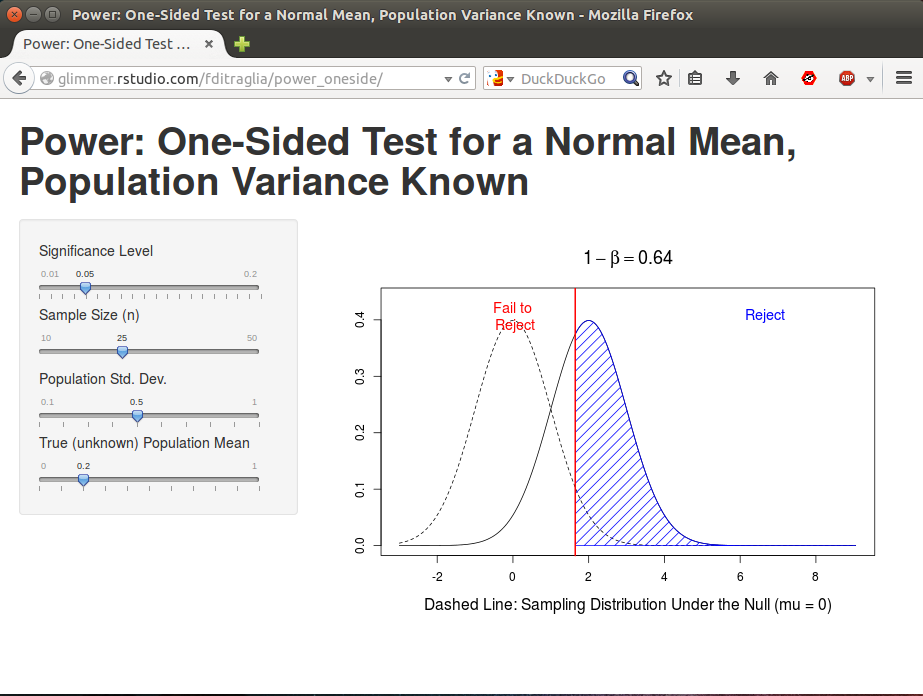
\includegraphics[scale = 0.3]{./images/power_oneside_screenshot}}
\end{figure}

\end{frame}
%%%%%%%%%%%%%%%%%%%%%%%%%%%%%%%%%%%%%%%%
\begin{frame}
	\frametitle{Power of Two-Sided Test}
\footnotesize
\begin{block}
	{Under the Alternative}
	$T_n = \sqrt{n}(\bar{X}_n/\sigma) \sim N\left( \sqrt{n}(\mu/\sigma),1  \right)$
\end{block}
\begin{block}
	{Decision Rule}
	Reject $H_0\colon \mu = 0$ if $|T_n|> \texttt{qnorm}(1- \alpha)$  
\end{block}
\begin{eqnarray*}
	1 - \beta &=& P(\mbox{Reject } H_0|H_0 \mbox{ false}) \pause = P(|T_n| >\texttt{qnorm}(1- \alpha/2))\\ \pause
		&=&\underbrace{P(T_n < -\texttt{qnorm}(1- \alpha/2)}_{\text{\alert{Lower}}} + \underbrace{P(T_n >\texttt{qnorm}(1- \alpha/2)}_{\text{\alert{Upper}}}\\ \\ \pause
	\mbox{\alert{Upper}} &=& (\mbox{Power of One-Sided Test with } \alpha/2 \mbox{ instead of } \alpha)\\ \pause
		&=& 1 - \texttt{pnorm}\left( \texttt{qnorm}(1 - \alpha/2) - \sqrt{n}(\mu/\sigma) \right) \\ \\ \pause
	\mbox{\alert{Lower}} &=& \texttt{pnorm}\left(-\texttt{qnorm}(1 - \alpha/2) - \sqrt{n}(\mu/\sigma) \right) \\
\end{eqnarray*}

\end{frame}
%%%%%%%%%%%%%%%%%%%%%%%%%%%%%%%%%%%%%%%%
\begin{frame}
	\frametitle{\href{https://fditraglia.shinyapps.io/power_twoside}{https://fditraglia.shinyapps.io/power\_twoside}}

\begin{figure}
	\fbox{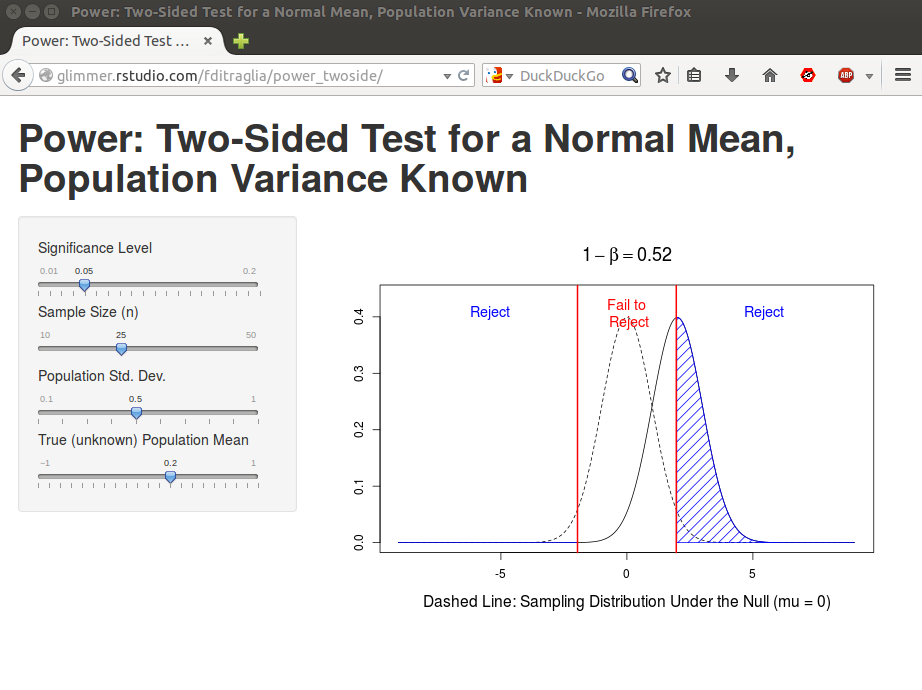
\includegraphics[scale = 0.3]{./images/power_twoside_screenshot}}
\end{figure}

\end{frame}
%%%%%%%%%%%%%%%%%%%%%%%%%%%%%%%%%%%%%%%%
\begin{frame}
\frametitle{What Determines Power?}
	\begin{block}{Power $ = 1 -  P$(Type II Error)}
Chance of detecting an effect given that one exists.
\end{block}
\begin{block}{Depends On:}
	\begin{enumerate}
\item Magnitude of Effect: \emph{true} value of $\mu$
	\begin{itemize}
		\item Easier to detect large deviations from $H_0\colon \mu = 0$
	\end{itemize}
\item Amount of variability in the population: $\sigma$
	\begin{itemize}
		\item Lower $\sigma \Rightarrow$ easier to detect effect of given magnitude
	\end{itemize}
\item Sample Size: $n$
\begin{itemize}
	\item Larger sample size $\Rightarrow$ easier to detect effect of given magnitude 
\end{itemize}
\item Significance Level: $\alpha$
\begin{itemize}
	\item Fewer Type I errors $\Rightarrow$ more Type II errors
\end{itemize}
\end{enumerate}
\end{block}

\end{frame}

%%%%%%%%%%%%%%%%%%%%%%%%%%%%%%%%%%%%%%%%%
\begin{frame}
\frametitle{Study Tip}
		Compare determinants of \emph{width} of $(1- \alpha)\times100\%$ CI to determinants of \emph{power} of corresponding two-sided test.
\end{frame}
%%%%%%%%%%%%%%%%%%%%%%%%%%%%%%%%%%%%%%%%%
\begin{frame}
\begin{center}
	\huge Some Final Thoughts on Hypothesis Testing and Confidence Intervals
\end{center}
\end{frame}
%%%%%%%%%%%%%%%%%%%%%%%%%%%%%%%%%%%%%%%%
\begin{frame}
\frametitle{Terminology I Have Intentionally Avoided Until Now}

\begin{block}{Statistical Significance}
Suppose we carry out a hypothesis test at the $\alpha\%$ level and,  based on our data, reject the null. You will often see this situation described as ``statistical significance.''
\end{block}

\begin{block}{In Other Words...}
When people say ``statistically significant'' what they really mean is that they rejected the null hypothesis.
\end{block}
\end{frame}

%%%%%%%%%%%%%%%%%%%%%%%%%%%%%%%%%%%%%%%
\begin{frame}
\frametitle{Some Examples}

	\begin{itemize}
		\item We found a difference between the ``Hi'' and ``Lo'' groups in the anchoring experiment that was statistically significant at the 5\% level based on data from a past semester.
		\item Our 95\% CI for the proportion of US voters who know who John Roberts is did not include 0.5. Viewed as a two-sided test, we found that the difference between the true population proportion and 0.5 was statistically significant at the 5\% level.
	\end{itemize}

\end{frame}
%%%%%%%%%%%%%%%%%%%%%%%%%%%%%%%%%%%%%%%
\begin{frame}
\frametitle{Why Did I Avoid this Terminology?}
\small
\begin{block}{Statistical Significance $\neq$ Practical Importance}
	\begin{itemize}
		\item You need to understand the term ``statistically significant'' since it is widely used. A better term for the idea, however, would be ``statistically discernible''
		\item Unfortunately, many people are confused about ``significance'' in the narrow, technical sense with the everyday English word meaning ``important'' 
		\item \alert{Statistically Significant Does Not Mean Important!"}
			\begin{itemize}
				\item A difference can be practically unimportant but statistically significant.
				\item A difference can be practically important but statistically insignificant.
			\end{itemize}
	\end{itemize}
\end{block}


\end{frame}


%%%%%%%%%%%%%%%%%%%%%%%%%%%%%%%%%%%%%%%
\begin{frame}
\begin{center}
\Huge P-value Measures Strength of Evidence Against $H_0$\\ \alert{Not The Size of an Effect!}
\end{center}
\end{frame}
%%%%%%%%%%%%%%%%%%%%%%%%%%%%%%%%%%%%%%%
\begin{frame}
\frametitle{Statistically Significant but Not Practically Important}
\small
I flipped a coin 10 million times (in R) and got 4990615 heads.
\begin{block}{Test of $H_0\colon p = 0.5$ against $H_1\colon p \neq 0.5$}
$$T = \displaystyle \frac{\widehat{p} - 0.5}{\sqrt{0.5(1-0.5)/n}} \approx -5.9   \implies \alert{\mbox{ p-value } \approx 0.000000003}$$
\end{block}

\begin{block}{Approximate 95\% Confidence Interval}
 $$\widehat{p} \pm \texttt{qnorm}(1 - 0.05/2) \sqrt{\frac{\widehat{p}(1-\widehat{p})}{n}}  \implies \alert{(0.4988, 0.4994)}$$
\end{block}

%\footnotesize (Such a huge sample size that refined vs.\ textbook CI makes no difference)
\large
\vspace{1em}

\alert{\fbox{Actual $p$ was 0.499}}
\end{frame}

%%%%%%%%%%%%%%%%%%%%%%%%%%%%%%%%%%%%%%%

\begin{frame}
\frametitle{Practically Important But Not Statistically Significant}
\framesubtitle{\href{http://www.amazon.com/p-value-Stories-Actually-Understand-Statistics/dp/0321629302}{\fbox{Vickers: ``What is a P-value Anyway?'' (p. 62)}}}
\footnotesize
\begin{quote}
Just before I started writing this book, a study was published reporting about a 10\% lower rate of breast cancer in women who were advised to eat less fat. If this is indeed the true difference, low fat diets could reduce the incidence of breast cancer by tens of thousands of women each year -- astonishing health benefit for something as simple and inexpensive as cutting down on fatty foods. The p-value for the difference in cancer rates was 0.07 and here is the key point: this was widely misinterpreted as indicating that low fat diets don't work. For example, the \emph{New York Times} editorial page trumpeted that ``low fat diets flub a test'' and claimed that the study provided ``strong evidence that the war against all fats was mostly in vain.'' \alert{However failure to prove that a treatment is effective is not the same as proving it ineffective.}
\end{quote}
\end{frame}
%%%%%%%%%%%%%%%%%%%%%%%%%%%%%%%%%%%%%%%
%\begin{frame}[c]\frametitle{Do Students with 4-Letter Surnames Do Better?}
 %\framesubtitle{Based on Data from Midterm 1 Last Semester}
   % \begin{columns}
    %	\column{0.35\textwidth} \begin{block}
    		%{4-Letter Surname}
    		%	$\bar{x} = 88.9$\\
    		%	$s_x = 10.4$\\
    		%	$n_x = 12$
   % 	\end{block} 
    %	\column{0.35\textwidth} \begin{block}
    	%	{Other Surnames}
    		%	$\bar{y} = 74.4$\\
    			%$s_y = 20.7$\\
    	%		$n_y = 92$
   % 	\end{block}
   % \end{columns}

%\vspace{1em}
%\begin{block}
%	{Difference of Means}
%	$\bar{x} - \bar{y} = \alert{14.5}$
%\end{block}
%\begin{block}
%	{Standard Error}
%	$\displaystyle SE = \sqrt{s_x^2/n_x + s_y^2/n_y} \approx \alert{3.7}$
%\end{block}
%\begin{block}
%	{Test Statistic}
%	$T = 14.5 / 3.7 \approx \alert{3.9}$
%\end{block}
%\end{frame}
%%%%%%%%%%%%%%%%%%%%%%%%%%%%%%%%%%%%%%%
%\begin{frame}[c]\frametitle{What is the p-value for the two-sided test?  \hfill 
\includegraphics[scale = 0.05]{./images/clicker}}
    
%$$\boxed{\mbox{Test Statistic} \approx 3.9}$$

%\begin{enumerate}[(a)]
%	\item $p < 0.01$
	%\item $0.01 \leq p < 0.05$
%	\item $0.05 \leq p < 0.1$
%	\item $p > 0.1$
%	\item Not Sure
%\end{enumerate}
%\end{frame}
%%%%%%%%%%%%%%%%%%%%%%%%%%%%%%%%%%%%%%%
%\begin{frame}[c]\frametitle{What do these results mean? \hfill 
\includegraphics[scale = 0.05]{./images/clicker}}

%Evaulate this statement in light of our hypothesis test:
%\vspace{1em}

%\begin{quote}
	%Students with four-letter long surnames do better, on average, on the first midterm of Econ 103 at UPenn.
%\end{quote}

%\begin{enumerate}[(a)]
%	\item Strong evidence in favor
%	\item Moderate evidence in favor
%	\item No evidence either way
%	\item Moderate evidence against
%	\item Strong evidence against
%\end{enumerate}
%\end{frame}
%%%%%%%%%%%%%%%%%%%%%%%%%%%%%%%%%%%%%%%
%\begin{frame}[c,fragile]\frametitle{I just did 134 Hypothesis Tests...}
   
 %\begin{block}
 %	{... and 11 of them were significant at the 5\% level.}
 %\end{block}

%\footnotesize

%\begin{verbatim}
  %       group sign p.value x.bar N.x  s.x y.bar N.y  s.y
%26  first1 = P    1   0.000  93.8   3  2.9  75.5 101 20.4
%70     id2 = 7    1   0.000  94.6   5  3.3  75.1  99 20.4
%134    id8 = 0    1   0.000  92.6   7  4.9  74.8  97 20.5
%5    Nlast = 4    1   0.001  88.9  12 10.4  74.4  92 20.7
%90     id4 = 8    1   0.003  87.7   9  9.0  74.9  95 20.7
%105    id6 = 8    1   0.003  88.1   5  5.8  75.4  99 20.6
%109    id6 = 2    1   0.007  88.9   8 10.7  75.0  96 20.6
%9    Nlast = 2    1   0.016  90.4   5  9.3  75.3  99 20.5
%49   last1 = P   -1   0.036  65.2   6  9.9  76.7  98 20.6
%65     id2 = 1    1   0.038  84.3   9 10.1  75.3  95 20.9
%117    id7 = 8    1   0.041  83.4  13 11.6  75.0  91 21.1
%\end{verbatim}
%\end{frame}


%%%%%%%%%%%%%%%%%%%%%%%%%%%%%%%%%%%%%%%%
\begin{frame}
\frametitle{Data-Dredging}
\begin{itemize}
	\item Suppose you have a long list of null hypotheses and assume, for the sake of argument that all of them are true.
		\begin{itemize}
			\item E.g.\ there's no difference in grades between students with different 4th digits of their student id number. 
		\end{itemize}
	\item We'll still reject about 5\% of the null hypotheses.
	\item Academic journals tend only to publish results in which a null hypothesis is rejected at the 5\% level or lower. 
	\item We end up with the bizarre result that ``most published studies are false.''  
\end{itemize}


\alert{To learn more:\quad \href{http://www.economist.com/news/briefing/21588057-scientists-think-science-self-correcting-alarming-degree-it-not-trouble}{\textcolor{blue}{\fbox{The Economist - "Trouble in the Lab.''}}}}


\end{frame}
%%%%%%%%%%%%%%%%%%%%%%%%%%%%%%%%%%%%%%%%
\begin{frame}
\frametitle{Green Jelly Beans Cause Acne!}
\framesubtitle{\href{http://xkcd.com/882/}{\fbox{xkcd \#882}}}
\begin{figure}
\centering
	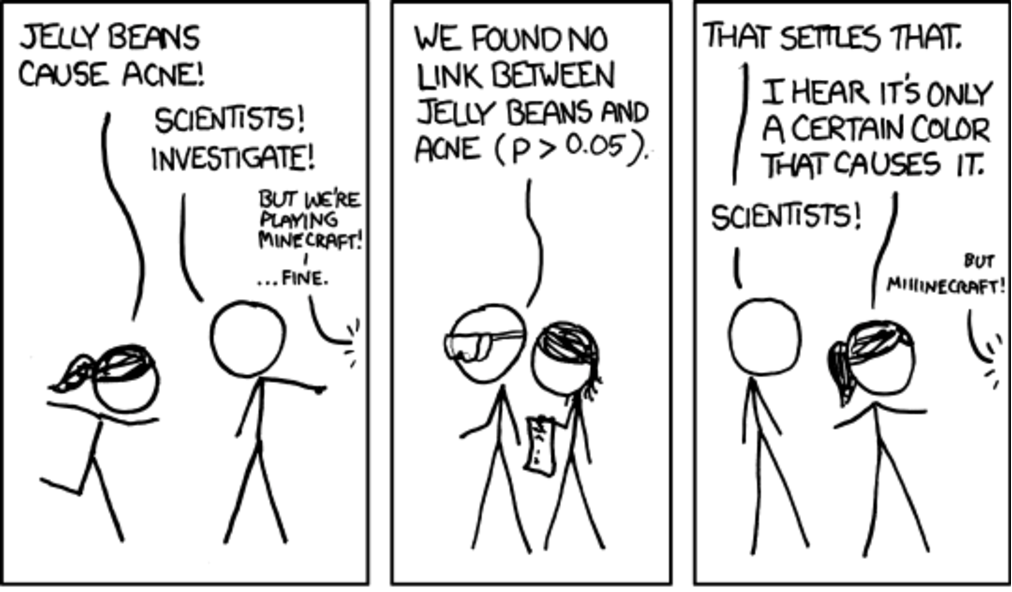
\includegraphics[scale=0.45]{./images/xkcd1}
	\caption{Go and read this comic strip: before today's lecture you wouldn't have gotten the joke!}
\end{figure}
\end{frame}
%%%%%%%%%%%%%%%%%%%%%%%%%%%%%%%%%%%%%%%%%
% \begin{frame}
% \frametitle{Don't Compare P-Values Across Different Tests!}
% \framesubtitle{\fbox{\href{http://www.people-press.org/files/2012/08/8-10-12-Knowledge-release.pdf}{Pew: ``What Voters Know About Campaign 2012''}}}


% \footnotesize

% Of 239 Republicans, 61\% knew Romney is pro-life vs.\ 53\% of 238 Democrats.
% \pause
% \begin{block}{$H_0\colon p_{Rep} = 0.5$ vs.\ $H_1\colon p_{Rep} \neq 0.5$}
%  $$T = \frac{0.61 - 0.5}{\sqrt{0.5(1-0.5)/239}} \approx  3.4 \implies \mbox{ p-value } \approx 0.0007$$
% \end{block}
% \pause
% \begin{block}{$H_0\colon q_{Dem} = 0.5$ vs.\ $H_1\colon q_{Dem} \neq 0.5$}
%  $$T = \frac{0.53 - 0.5}{\sqrt{0.5(1-0.5)/238}} \approx 0.93  \implies \mbox{ p-value } \approx 0.35$$
% \end{block}
% \pause
% \begin{block}{$H_0\colon p_{Rep} =q_{Dem}$ vs.\ $H_1\colon p_{Rep} \neq q_{Dem}$}
%  $$T = \frac{0.61 - 0.53}{\sqrt{\left(\frac{1}{239}+ \frac{1}{238}\right)\left(\frac{239 \times 0.61 + 238 \times 0.53}{239 + 238}\right)}} \approx  1.76 \implies \mbox{ p-value } \approx 0.08$$
% \end{block}


% \end{frame}

% %%%%%%%%%%%%%%%%%%%%%%%%%%%%%%%%%%%%%%%%
% \begin{frame}
% \frametitle{Don't Compare P-Values Across Different Tests!}

% \begin{itemize}
% 	\item P-Value measures strength of evidence against the null, not the size of an affect! \pause
% 	\item Use a single test to address a single research question: if you are actually interested in differences between Republicans and Democrats, test for this directly! \pause
% \end{itemize}

% \vspace{1em}

% \pause

% For more on the problems associated with comparing p-values from different hypothesis tests, along with an even starker example than the one I just showed you, see \href{http://amstat.tandfonline.com/doi/abs/10.1198/000313006X152649}{\textcolor{blue}{\fbox{Gelman \& Stern (2006)}}}

% \end{frame}
% %%%%%%%%%%%%%%%%%%%%%%%%%%%%%%%%%%%%%%%%%

\begin{frame}
\frametitle{Some Final Thoughts}
	\begin{itemize}
		\item Failing to reject $H_0$ does not mean $H_0$ is true. 
		\item Rejecting $H_0$ does not mean $H_1$ is true.
		\item P-values are always more informative than simply reporting ``Reject'' vs.\ ``Fail To Reject'' at a given significance level. 
		\item Confidence intervals are informative since they give an idea of the size of an effect. 
%		\item If $H_0$ is actually plausible a priori (this is rarer than you may think), reporting a p-value can be a good complement to a CI. 
		\item To avoid data-dredging, be honest about the tests you have carried out: report \emph{all of them}, not just the ones where you rejected the null.
	\end{itemize}

\end{frame}
\end{document}
